\begin{markdown}
#30天 LaTeX 挑戰 Day 22 pgfplots

------

pgfplots 是一個可以畫出複雜的三維圖表的強大 Package,需要注意的是這個 Package 是基於前面介紹過的 Ti*k*Z,所以在使用之前請記得要先使用 Ti*k*Z。

##簡介

在使用 pgfplots 之前我們需要先使用 tikzpicture 環境,之後再使用 pgfplots  提供的 axis 環境。

```latex
\begin{tikzpicture}
\begin{axis}
......
\end{axis}
\end{tikzpicture}
```

我們要將 pgfplots 提供的命令放在 axis 環境中,第一個要介紹的是 `\addplot[可選參數]{方程式}` 這個命令,大部分可選參數是與 Ti*k*Z 的可選參數相同,方程式則是與大部分程式語言的表達方式一樣。

```latex
\begin{tikzpicture}
\begin{axis}
\addplot[domain=-5:5, color=blue] {x^2};
\end{axis}
\end{tikzpicture}
```

使用完之後也請不要忘記在最後面加上 ;。

##二維圖形

###函數圖

第一個介紹的還是函數圖,簡單的範例上面展示過了,所以這裡會比較注重在介紹不同的可選參數。

```latex
\begin{tikzpicture}
\begin{axis}
\addplot[domain=-5:5, color=blue] {x^2};
\end{axis}
\end{tikzpicture}
```

這是上面所展示的陽春例子,我們可以在多加一個方程式讓他看起來好一點。

```latex
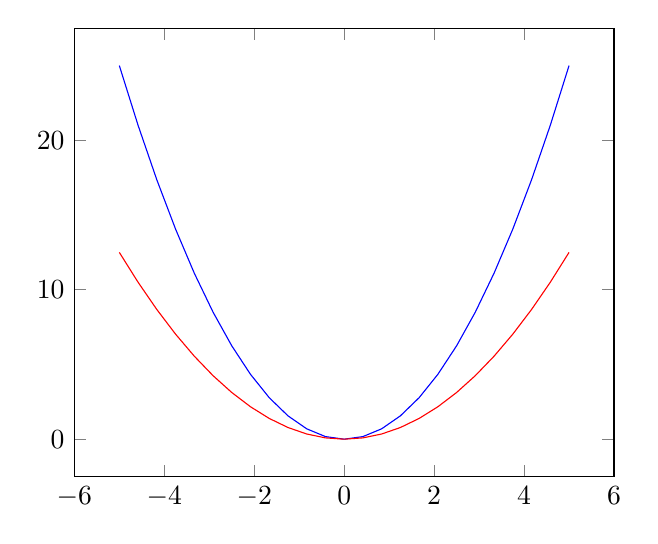
\begin{tikzpicture}
\begin{axis}
\addplot[domain=-5:5, color=blue] {x^2};
\addplot[domain=-5:5, color=red] {x^2/2};
\end{axis}
\end{tikzpicture}
```

可是這樣沒有標示難免會讓人搞混,所以我們可以利用 `\addlegendentry ` 加入註解。

```latex
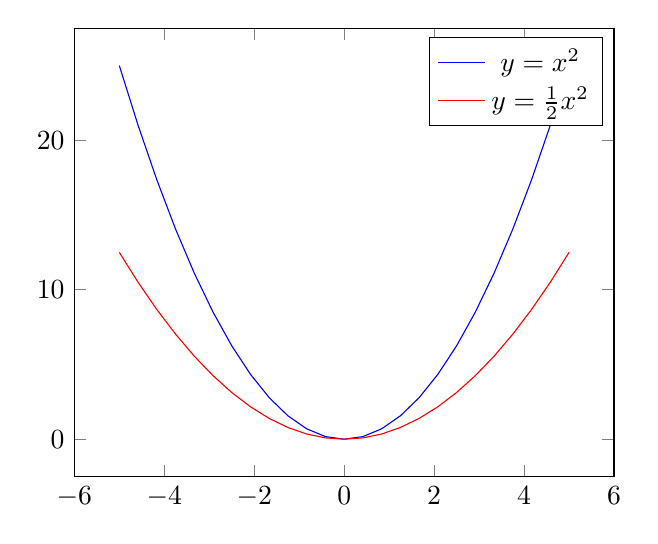
\begin{tikzpicture}
\begin{axis}
\addplot[domain=-5:5, color=blue] {x^2};
\addlegendentry{\(y=x^2\)}
\addplot[domain=-5:5, color=red] {x^2/2};
\addlegendentry{\(y=\frac{1}{2}x^2\)}
\end{axis}
\end{tikzpicture}
```

這樣就不會搞混了,如果今天想要用對數來當 x, y 軸的單位,pgfplots 也有提供 `\begin{semilogxaxis}` 與 `\begin{semilogyaxis}` 來解決這個問題。

```latex
\begin{tikzpicture}
\begin{semilogyaxis}
\addplot[domain=-10:10, color=blue, samples=1000] {log10(x)};
\end{semilogyaxis}
\end{tikzpicture}
```

有時候座標軸會不符合我們想要的樣式,這時可以利用 axis lines 來調整。

```latex
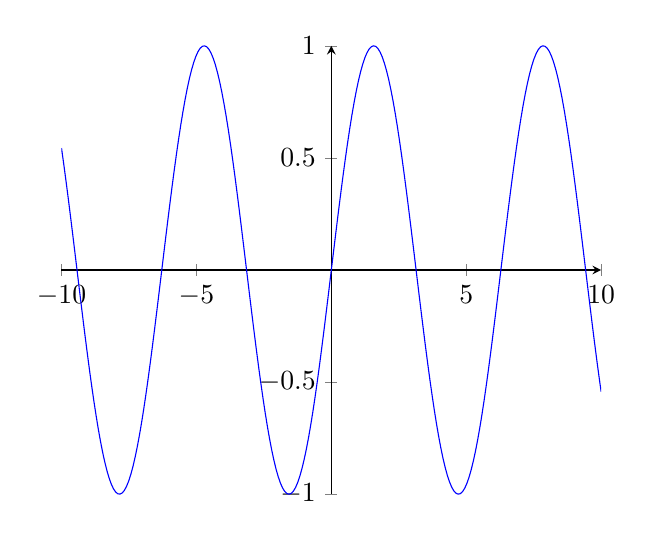
\begin{tikzpicture}
\begin{axis}[axis lines = middle]
\addplot[domain=-10:10, color=blue, samples=250] {sin(deg(x))};
\end{axis}
\end{tikzpicture}
```

\end{markdown}